\section{Evaluation}

\subsection{Trend analysis evaluation}
To evaluate our result, we first try to show that our trend analysis
works well. To do that, we collect other document with topic label.
With these test set, its trend analysis result indirectly shows our
accuracy of trend analysis.
\subsection{Selecting test set}
We use reuters data set. It consists of more than 9000 documents
with more than 70 topics. But, the similarity of document is important
because evaluation on very diffrent set of documents doesn't imply
any meaningful result. To resolve that, we decided to extract 10 topics
with most similarity between our dataset. It is achieved by calculating
document similarity between reuters dataset and our news dataset.

To pick most similar topic, we compute maximum similarity within documents
in topic and minimum similarity between reuters and news dataset. Due to
largeness of dataset, we choose only subset of dataset to calculate
minimum/maximum similarity bewteen groups. Similarity of groups are
represented as graph in figure \ref{fig:distance}. Distance of nearest
10 topics in reuters dataset is shown as table \ref{table:topicdistance}.
Also, there are significant difference of distances between nearest group and
others, as shown as table \ref{table:groupdistance}.

\subsection{Reuters evaluation}
With reuters dataset with 10 pre-classified topics, we generate LDA
model for reuters dataset and make 10 topics. And we classified the topic
with given label. In result, we successfully classified 7 topics from
LDA result. It shows that our LDA model seems to work correctly. Precise
result is shown as table \ref{table:matchedtopic}.

\begin{figure}[!htbp]
  \centering
  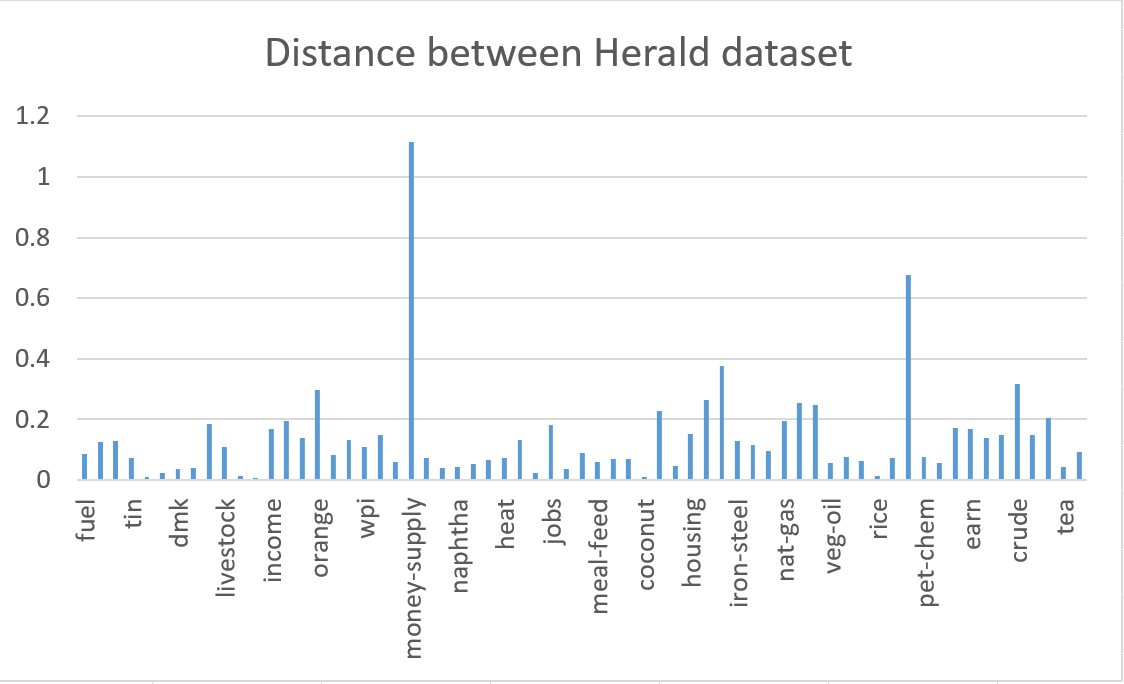
\includegraphics[width=0.8\linewidth]{Distance1}
  \caption{Distance between Herald dataset.}
  \label{fig:distance}
\end{figure}

\begin{table}[!htbp]
  \begin{tabular}{l|l}
  Topic & distance \\ \hline
  yen & 0.0061 \\
  lumber & 0.0524 \\
  veg-oil & 0.0566 \\
  strategic-metal & 0.0576 \\
  carcass & 0.0593 \\
  metal-feed & 0.0606 \\
  gold & 0.0622 \\
  ship & 0.0681 \\
  cocoa & 0.0718 \\
  oilseed & 0.0731
  \end{tabular}
  \caption{Distance of nearest 10 topics between Herald dataset.}
  \label{table:topicdistance}
\end{table}

we think that this evaluation is meaningful becuase the evaluation was conducted on
well-known external \textbf{labeled} dataset sources, which proves the objectivity
of the evaluation. In other words, this evaluation was not just done by manual
judgement. Also, among those reuters datasets, we only evaluated those
that showed close similarity values(similar trends) with our Herald dataset, thus increasing the
accuracy.


\begin{table}[!htbp]
  \begin{tabular}{l|l}
  Group & distance \\ \hline
  nearest 10 topics & 0.061 \\
  other topics & 0.1964
  \end{tabular}
  \caption{Difference between nearest topics and another.}
  \label{table:groupdistance}
\end{table}

\begin{table}[!htbp]
  \begin{tabular}{l|l}
      Topic & matched label \\ \hline
      0 & Unknown \\
      1 & oilseed \\
      2 & veg-oil \\
      3 & gold \\
      4 & Unknown \\
      5 & Unknown \\
      6 & lumber \\
      7 & yen \\
      8 & oilseed \\
      9 & cocoa \\
  \end{tabular}
  \caption{Matched topic and label.}
  \label{table:matchedtopic}
\end{table}



\subsection{Off-issue tracking}

For off-issue tracking, we just evaluated dunn index of clusters for many epsilon values of DBSCAN algorithm.
If dunn index is high, then it means cluster has higher distance between cluster, and has lower distance in cluster.
The result shows that smaller epsilon makes greater dunn index, but number of cluster is decreasing. So,
we have to decide appropriate epsilon value for better result. Numerical result of calculation is shown as table \ref{table:dunnindex}.
\begin{table}[!htbp]
  \begin{tabular}{l|l|l|l|l}
  Epsilon   & $\max \Delta_{k}$ & $\min \delta(C_{i}, C_{j})$ & $DI_{m}$ & \# of cluster \\ \hline
  3 &  8.122 & 192.0 & 24.26 & 5 \\
  5 &  22.23 & 163.2 & 7.34 & 12 \\
  7 &  52.72 & 138.4 & 2.625 & 16  \\
  9 & 106.7 & 102.1 & 0.9564 & 28
  \end{tabular}
  \caption{Dunn index and number of cluster for internal evaluation.}
  \label{table:dunnindex}
\end{table}
